% !TEX TS-program = Xelatex
% !TEX encoding = UTF-8 Unicode

\documentclass[UTF8,size=9.5]{ctexart}
\usepackage{amsmath}
\usepackage{dsfont}
\usepackage[table]{xcolor}
\usepackage[bottom]{footmisc}
\usepackage{graphicx}
\usepackage{hyperref}
\usepackage{enumitem}
\usepackage{figsize}
\usepackage{standalone}
\usepackage[separate-uncertainty = true,tight-spacing=true,round-minimum=0.00000000001]{siunitx}
\usepackage{tabu}
\usepackage{wasysym}
\usepackage{geometry}
\geometry{left=0.7in,right=0.7in,bottom=0.7in,top=0.7in}

\title{计算物理学作业4}
\author{朱寅杰 1600017721}
\date{}
\begin{document}

\maketitle
\setcounter{section}{4}
\subsection{求解Lotka–Volterra方程的初值问题}
对于微分方程组
\begin{equation}(\dot{x},\dot{y})=(\alpha x-\beta xy,\delta xy-\gamma y)\end{equation}
作变量代换$(X,Y,T)=(\delta x/\alpha,\beta y/\alpha,\alpha t)$,得到
\begin{equation}(\dot{X},\dot{Y})=(X(1-Y),Y(X-\gamma/\alpha)),\gamma/\alpha>0\end{equation}

对于这个方程组,我们首先考察其不含时的不动点解(即$\dot{X}=\dot{Y}=0$的解):其一为$X(T)=Y(T)=0$,其一为$X(T)=\gamma/\alpha,Y(T)=1$。作一个微扰的话,
\begin{enumerate}[label={\alph*)},font=\bfseries]
\item
对于前者,设$X(T)=\epsilon_1(T)$,$Y(T)=\epsilon_2(T)$,其中$\epsilon$均为小量。从而有
$(\dot{\epsilon_1},\dot{\epsilon_2})= (\epsilon_1(1-\epsilon_2),(\epsilon_1-\gamma/\alpha)\epsilon_2)$,再对$T$求导,并保留至最低阶小量,有
\[(\ddot{\epsilon_1},\ddot{\epsilon_2})=\bigl(\epsilon_1(1-\epsilon_2)^2-\epsilon_1\epsilon_2(1-\gamma/\alpha),\epsilon_2(\epsilon_1-\gamma/\alpha)^2+\epsilon_1\epsilon_2(1-\epsilon_2)\bigr)\approx(\epsilon_1,-(\gamma/\alpha)^2\epsilon_2)\]

也就是说对于$X$方向上的微扰这个不动点是不稳定的,而对于$Y$方向上的微扰这个不动点是稳定的。
\item
对于后者,取$X(T)=\gamma/\alpha+\epsilon_1(T),Y(0)=1+\epsilon_2(T)$,则有
\[(\dot{\epsilon_1},\dot{\epsilon_2})=\bigl(-(\epsilon_1+\gamma/\alpha)\epsilon_2,(1+\epsilon_2)\epsilon_1\bigr)\]
再对$T$求导,保留至一阶小量,得到
\[(\ddot{\epsilon_1},\ddot{\epsilon_2})=\bigl(-(\epsilon_1+\gamma/\alpha)(1+\epsilon_2)\epsilon_1,\epsilon_1^2(1+\epsilon_2)-(1+\epsilon_2)(\epsilon_1+\gamma/\alpha)\epsilon_2\bigr)\approx(-\epsilon_1\gamma/\alpha,-\epsilon_2\gamma/\alpha)\]
故这是一个稳定不动点。
\end{enumerate}

事实上,这个微分方程组是可积的。将两式相除得到
\[\frac{\mathrm{d}Y}{\mathrm{d}X}=\frac{Y(X-\gamma/\alpha)}{X(1-Y)}\]
分离变量积分得到$X+Y-\log{(X^{\gamma/\alpha}Y)}=$常数。写作变量代换之前的形式,就是$\delta x+\beta y-\gamma\log{x}-\alpha\log{y}=$常数。

最后,我们使用 Runge-Kutta法来数值求解这个问题中$\alpha=2/3,\beta=4/3,\gamma=\delta=1$的特殊情况。求解的代码见\href{./RK.py}{RK.py}。总共计算了$(x,y)=(0.8,0.8)$、$(1.0,1.0)$、$(1.2,1.2)$、$(1,4,1.4)$、$(1.6,1.6)$五组初值的解,将五个初值下$(x,y)$的演化轨迹一并画在下图中。从图中可见,这几个初值解出的都是围绕着不动点$(x,y)=(1.0,0.5)$(对应于$(X,Y)=(\gamma/\alpha,1)$)逆时针走行的闭合曲线,而这闭合曲线正是上面求出的这个微分方程组的初积分的等值线。

\begin{figure}
  \centering
  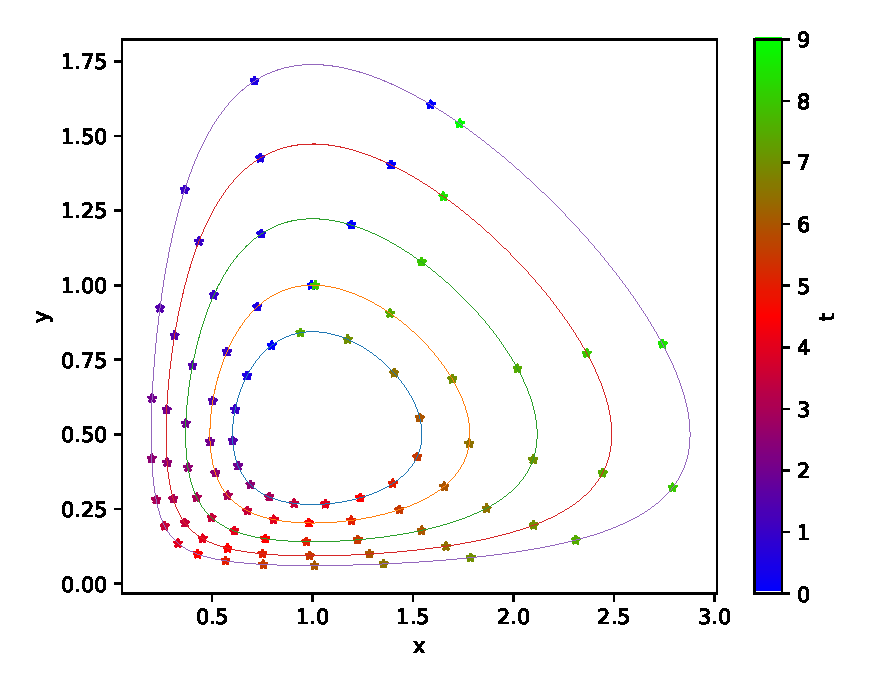
\includegraphics[width=\linewidth]{RK.eps}
  \caption{图中由内至外分别是初值为$(x,y)= (0.8,0.8),(1.0,1.0),(1.2,1.2),(1,4,1.4),(1.6,1.6)$的解以参数方程的方式画出的曲线。为了标示$(x,y)$随$t$的演化规律,从$t=0$开始,每隔0.5在图线上的$(x(t),y(t)$处打一个节点,直至图线转过一周。不同的$t$对应的点的颜色是由蓝到红到绿渐变的,所以如果你对色彩的敏感度足够高,就可以直接通过颜色(而不用从初始点开始一个一个数)来确定在$t$为某值时各个解都演化到什么地方了。图片是矢量图,因此如果想要观察细节可以尽情地zoom in。}
\end{figure}

\subsection{不同的稀疏矩阵迭代法求解泊松方程边值问题的速度比较}
待解的方程是
\[-\nabla^2u(x,y)=2\pi^2\sin(\pi x)\sin(\pi y),(x,y)\in(0,1)\times(0,1)\]
并且给出在边界上函数的值为零。将待解的区域分割成$h=\frac{1}{N+1}$见方的方格,把算子$\nabla^2$作分立化处理,求解在格点上的$N\times N$个函数值。这实际上就变成了一个稀疏矩阵的线性方程组的求解问题,可以使用迭代进行求解。

我们分别使用了Jacobi法、Gauss-Seidel法和经过Chebyshef加速的弛豫算法(感谢刘老师的讲义,弛豫算法与Chebyshef加速中需要计算的谱半径等参数都已经帮我们算好了,只需拿来使用即可)来进行求解,并统计其迭代次数。为便于比较,迭代停止的标准统一选作各格点处方程左右两边差的绝对值不超过\num{e-4}。计算的源代码分别为\href{./Jacobi.py}{Jacobi.py}、\href{./Gauss-Seidel.py}{Gauss-Seidel.py}和\href{./SOR.py}{SOR.py}。分别计算了$N=10,20,...,60$的情况(虽然题目里只要求算了10、20和50),结果列于下表中:
\begin{center}
\begin{tabu} to \linewidth {X[c]|X[c]X[c]|X[c]X[c]|X[c]X[c]}
\hline
	&\multicolumn{2}{c|}{Jacobi}&\multicolumn{2}{c|}{Gauss-Seidel}&\multicolumn{2}{c}{SOR}\\
$N$	&迭代步数	&$r_{max}$&迭代步数	&$r_{max}$&迭代步数	&$r_{max}$\\
\hline
10&  295& \num{9.745e-05}&  149& \num{9.413e-05}&  33& \num{7.310e-05}\\
20& 1086& \num{9.894e-05}&  544& \num{9.912e-05}&  63& \num{9.410e-05}\\
30& 2370& \num{9.994e-05}& 1187& \num{9.900e-05}&  94& \num{8.362e-05}\\
40& 4149& \num{9.996e-05}& 2076& \num{9.971e-05}& 124& \num{9.051e-05}\\
50& 6423& \num{9.981e-05}& 3213& \num{9.965e-05}& 154& \num{9.487e-05}\\
60& 9190& \num{9.991e-05}& 4596& \num{9.993e-05}& 184& \num{9.793e-05}\\
\hline
\end{tabu}
\end{center}
可以看到,Gauss-Seidel迭代所用次数几乎等于Jacobi迭代的一半,二者基本都以$N^2$的方式增长。而优化后的弛豫算法的迭代次数是随着$N$线性增长的(而且线性十分好)。如果进一步拟合的话可以发现,三者的增长规律分别是$2.4714(N+0.99)^2-3$、$1.235(N+1.01)^2-1$、$3.023(N+1)$,与理论预期符合得相当好。
\end{document}


